\documentclass[a4paper,11pt]{report}

% ---- Page layout ----
\usepackage[margin=2.5cm]{geometry}

% ---- Fonts (XeLaTeX) ----
\usepackage{fontspec}

% ---- Typography & links ----
\usepackage{microtype}
\usepackage{xcolor}
\usepackage{hyperref}
\hypersetup{
    colorlinks = true,
    linkcolor  = blue!50!black,
    citecolor  = blue!50!black,
    urlcolor   = blue!50!black
}

% ---- Math ----
\usepackage{amsmath,amssymb,mathtools}

% ---- Figures, tables, listings ----
\usepackage{graphicx}
\usepackage{float}
\usepackage{booktabs}
\usepackage{array}
\usepackage{caption}
\usepackage{subcaption}
\usepackage{pgfplots}
\pgfplotsset{compat=1.17}
\usepackage{listings}
\lstset{
    basicstyle=\ttfamily\small,
    breaklines=true,
    frame=single,
    language=Python,
    keywordstyle=\color{blue!60!black},
    commentstyle=\color{gray},
    columns=fullflexible
}

% ---- Header / footer ----
\usepackage{fancyhdr}
\pagestyle{fancy}
\fancyhf{}
\rfoot{\thepage}
\renewcommand{\headrulewidth}{0pt}

\begin{document}

\begin{titlepage}
    \centering
    \vspace*{3cm}

    {\LARGE\bfseries Sentiment Analysis of Amazon Fine Food Reviews}\\[0.4cm]
    {\Large A Three-Class Sentiment Classifier with Deep Learning}\\[2cm]

    \rule{0.8\linewidth}{0.6pt}\\[0.5cm]
    {\large Introduction to Deep Learning Project Report}\\[0.2cm]
    \rule{0.8\linewidth}{0.6pt}

    \vfill

    \begin{tabular}{ll}
        \textbf{Instructor:} & Dr. Trần Việt Trung \\
    \end{tabular}

    \vspace{0.8cm}

    \textbf{Student}\\[0.3cm]
    \begin{tabular}{ll}
        Nguyễn Tuệ Lâm & 20261207M \\
    \end{tabular}

    \vspace{1cm}
    {\large \today}

    \vspace*{1cm}
\end{titlepage}

\tableofcontents

\chapter{Introduction}
\label{ch:introduction}
\section{Project Background}
\label{sec:1-1}

Online shops receive thousands of product reviews every day. Reading them by hand is not feasible, yet the sentiment they carry tells a seller which products disappoint buyers and which are praised.

Turning that text into a signal that can be counted is difficult because a star rating and the words of a review do not always agree. A review titled \emph{``Not as Advertised''} that begins ``Product arrived labeled as Jumbo Salted Peanuts\ldots the peanuts were actually small sized unsalted'' is negative without containing a single strongly negative word. A classifier has to read the sentence, not count words.

This project uses the Amazon Fine Food Reviews corpus~\cite{mcauley2013,kaggle_fine_food}: 568{,}454 reviews posted between October 1999 and October 2012, each with a star rating. The ratings give labels without manual annotation, but they are skewed: after cleaning, about 78\% of the reviews are positive and only 7.6\% are neutral. A classifier that always answers \emph{positive} reaches about 78\% accuracy while recognising nothing about the other classes. Deep learning models that read the text in context are therefore tested on a problem where the obvious shortcut is already strong.

\section{Problem Statement}
\label{sec:1-2}

\begin{itemize}
    \item \textbf{Difficulty in reading sentiment from text.} Sentiment depends on negation (``not bad''), contrast (``good but\ldots'') and context, so counting words is not enough. Models must use word order and context.
    \item \textbf{Imbalanced and approximate labels.} The labels are derived from star ratings, not from human annotation, and the neutral class (3 stars) is rare and ambiguous. A model can look good on accuracy while failing on the minority classes.
\end{itemize}

\section{Research Questions}
\label{sec:1-3}

\begin{enumerate}
    \item How can raw reviews and star ratings be turned into a clean labelled corpus in which the same text never appears in both training and test data?
    \item How skewed are the classes and how long are the reviews, and what do these facts imply for the metric, the loss and the sequence length?
    \item How much does a pre-trained Transformer fine-tuned on this data (BERT) improve over a recurrent network trained from scratch (BiLSTM with attention)?
    \item How far do the two trained models improve on the rule that always answers \emph{positive}, and on which classes?
    \item Where do the models fail, in particular on the neutral class and on reviews whose text contradicts their rating?
\end{enumerate}

\section{Project Objectives}
\label{sec:1-4}

To build and compare deep learning classifiers that assign one of three sentiment labels (negative, neutral, positive) to the text of a food review, using a clean, leakage-safe dataset and an evaluation that is not fooled by the dominant positive class.

\section{Scope and Limitations}
\label{sec:1-5}

\textbf{In scope:} three-class sentiment classification of English review text, data cleaning and splitting, a BiLSTM with attention trained from scratch, a fine-tuned BERT encoder, and the always-positive rule as reference.

\textbf{Out of scope / not claimed:}
\begin{itemize}
    \item Human-annotated sentiment -- labels come from star ratings, so some are wrong by construction (Section~\ref{sec:2-2}).
    \item Predicting the sentiment of \emph{future} reviews -- the split is random, not chronological (Section~\ref{sec:5-8}).
    \item Aspect-level sentiment (which feature of the product is praised or criticised), other languages and other product domains.
    \item A deployed service.
\end{itemize}

\section{Report Structure}
\label{sec:1-6}

The report is organised into chapters that follow the order in which the work was built. The chapters are:

\begin{enumerate}
    \item \textbf{Introduction} -- background, problem statement, research questions, objectives and scope.
    \item \textbf{Problem Statement and Approach} (Chapter~\ref{ch:problem-approach}) -- weak labels, success criteria, metrics and the analytical approach.
    \item \textbf{Dataset and Data Specification} (Chapter~\ref{ch:dataset}) -- the Amazon Fine Food Reviews corpus, its schema, conventions and limitations.
    \item \textbf{Data Understanding} (Chapter~\ref{ch:data-understanding}) -- class distribution, text length, change over time, users, noise and vocabulary, and the design decisions they imply.
    \item \textbf{Data Preparation} (Chapter~\ref{ch:data-preparation}) -- cleaning, model input text, stratified split, fixed test subset and class weights.
    \item \textbf{Modeling} (Chapter~\ref{ch:modeling}) -- the BiLSTM with attention and the fine-tuned BERT.
    \item \textbf{Evaluation} (Chapter~\ref{ch:evaluation}) -- test results, confidence intervals, the neutral class, review length, threshold calibration, errors and limitations.
    \item \textbf{Conclusion} (Chapter~\ref{ch:conclusion}) -- summary, limitations, future work and reproducibility.
\end{enumerate}


\chapter{Problem Statement and Approach}
\label{ch:problem-approach}
\section{Review Platforms and Sentiment Monitoring}
\label{sec:2-1}

A shop that sells through an online marketplace receives feedback as free text. Each review shows how a customer felt about a product, and a collection of them shows which products are praised and which are criticised. Counting reviews by sentiment turns that text into a number that can be tracked over time and compared between products.

\section{Sentiment from Stars: Weak Labels}
\label{sec:2-2}

The dataset has no sentiment annotation, only the number of stars (1--5) chosen by the reviewer. The stars are used as a \textbf{weak label}: cheap to obtain but only approximately correct. The mapping is fixed once:

\begin{center}
\begin{tabular}{@{}lccccc@{}}
    \toprule
    Stars (\texttt{Score}) & 1 & 2 & 3 & 4 & 5 \\
    \midrule
    Label & negative & negative & neutral & positive & positive \\
    \bottomrule
\end{tabular}
\end{center}

A reviewer may give five stars and still write a complaint, so some labels are wrong by construction. This is treated as a property of the data, not hidden, and is examined when the errors of the models are analysed.

\section{Business Objectives}
\label{sec:2-3}

The objective is to classify the sentiment of a review from its text alone. The specific objectives are:

\begin{itemize}
    \item \textbf{Prepare a trustworthy dataset:} remove repeated reviews before splitting, so the evaluation measures generalisation and not memorisation.
    \item \textbf{Build two neural classifiers:} a BiLSTM with attention trained from scratch, and a BERT encoder fine-tuned on the same data.
    \item \textbf{Compare them fairly:} on identical test reviews, with an always-positive rule as reference.
\end{itemize}

\section{Evaluation Metrics}
\label{sec:2-4}

Accuracy is not a sufficient measure here, because always answering \emph{positive} already scores about 78\%. For each class $c$, precision, recall and F1 are
\begin{equation*}
    P_c = \frac{TP_c}{TP_c+FP_c},\qquad
    R_c = \frac{TP_c}{TP_c+FN_c},\qquad
    F1_c = \frac{2\,P_c R_c}{P_c+R_c},
\end{equation*}
and the main metric is \textbf{Macro-F1}, the unweighted mean over the three classes:
\begin{equation*}
    \text{Macro-F1} = \frac{1}{3}\sum_{c} F1_c .
\end{equation*}
Every class counts equally, so the small neutral class weighs as much as the large positive class. Accuracy, weighted F1, the F1 of each class, the confusion matrix, training time and parameter count are reported as well.

\section{Success Criteria}
\label{sec:2-5}

Success is defined \textbf{relative to simple alternatives} rather than by arbitrary absolute thresholds:

\begin{center}
\begin{tabular}{@{}p{3cm}p{11.5cm}@{}}
    \toprule
    Level & Criterion (evaluated on the unseen test part) \\
    \midrule
    Predictive & Each trained model has a higher Macro-F1 than the always-positive rule (about 0.29). \\
    Transfer learning & The fine-tuned BERT model has a higher Macro-F1 than the BiLSTM trained from scratch, and the paired bootstrap interval of the difference does not contain 0. \\
    Minority classes & The F1 of the negative and neutral classes is reported separately and is above 0 for every model. \\
    \bottomrule
\end{tabular}
\end{center}

\section{From Objective to Analytical Problem}
\label{sec:2-6}

The input is the English text of one review, made of a short title (\texttt{Summary}) and a body (\texttt{Text}). The output is one label $y \in \{\text{negative}, \text{neutral}, \text{positive}\}$. The task is to learn a function $f_\theta$ from text to $\{0,1,2\}$ by minimising a class-weighted cross-entropy loss on the training part (Section~\ref{sec:5-7}).

\section{Approach}
\label{sec:2-7}

\begin{center}
\begin{tabular}{@{}c@{}}
    \textbf{Raw Reviews} (568{,}454 rows) \\
    $\downarrow$ \\
    \textbf{Cleaning} -- remove repeated reviews and invalid rows \\
    $\downarrow$ \\
    \textbf{Input Text and Label} -- title $+$ body, label from stars \\
    $\downarrow$ \\
    \textbf{Stratified Split} -- train / validation / test, plus a fixed test subset \\
    $\downarrow$ \\
    \textbf{Training} -- BiLSTM with attention; BERT fine-tuning; class-weighted loss \\
    $\downarrow$ \\
    \textbf{Evaluation} -- Macro-F1, bootstrap intervals, error analysis \\
\end{tabular}
\end{center}

\section{Implementation Roadmap}
\label{sec:2-8}

The approach is implemented as a sequence of steps, each covered by one chapter:

\begin{itemize}
    \item \textbf{Specify the data} (Chapter~\ref{ch:dataset}) -- source, schema, conventions and what is not available.
    \item \textbf{Understand the data} (Chapter~\ref{ch:data-understanding}) -- class balance, length, time, noise, vocabulary; these set the metric, the sequence limits and the cleaning rules.
    \item \textbf{Prepare the data} (Chapter~\ref{ch:data-preparation}) -- clean, build the input text, split, and compute class weights.
    \item \textbf{Model and evaluate} -- BiLSTM with attention and BERT fine-tuning (Chapter~\ref{ch:modeling}) and the comparison of the models (Chapter~\ref{ch:evaluation}).
\end{itemize}


\chapter{Dataset and Data Specification}
\label{ch:dataset}
\section{Data Source and Collection}
\label{sec:3-1}

The project uses the publicly available \textbf{Amazon Fine Food Reviews} dataset, collected by McAuley and Leskovec~\cite{mcauley2013} and distributed on Kaggle~\cite{kaggle_fine_food}. It is a historical extract of food reviews posted on Amazon between October 1999 and October 2012. The dataset is read from a single CSV file of about 300~MB for inspection, cleaning and modelling.

\section{Dataset Characteristics and Limitations}
\label{sec:3-2}

\begin{itemize}
    \item \textbf{Weak labels.} The only sentiment signal is the star rating, which does not always agree with the text (Section~\ref{sec:2-2}).
    \item \textbf{Repeated reviews.} Amazon shares one review among the variants (flavours, sizes) of a product, so the same review appears under several product codes (Section~\ref{sec:5-2}).
    \item \textbf{One domain.} All reviews concern food products, so results do not necessarily carry over to electronics, books or films.
    \item \textbf{Change over time.} The volume, average rating and share of negative reviews all change between 2003 and 2012 (Section~\ref{sec:4-5}).
\end{itemize}

\section{Raw Data Schema}
\label{sec:3-3}

The raw dataset is a single flat table of 568{,}454 rows and 10 columns; each row is one review.

\begin{center}
\begin{tabular}{@{}p{4.6cm}p{2cm}p{8cm}@{}}
    \toprule
    Column & Type & Description \\
    \midrule
    \texttt{Id} & integer & Row number. \\
    \texttt{ProductId} & string & Product code. \\
    \texttt{UserId} & string & User code. \\
    \texttt{ProfileName} & string & User display name; missing in 26 rows. \\
    \texttt{HelpfulnessNumerator} & integer & Number of readers who found the review helpful. \\
    \texttt{HelpfulnessDenominator} & integer & Number of readers who voted at all (helpful or not). \\
    \texttt{Score} & integer & Star rating from 1 to 5; the source of the label. \\
    \texttt{Time} & integer & Posting time as a Unix timestamp. \\
    \texttt{Summary} & string & Short review title; missing in 27 rows. \\
    \texttt{Text} & string & Review body; complete. \\
    \bottomrule
\end{tabular}
\end{center}

\section{Pipeline Column Names}
\label{sec:3-4}

The raw columns keep their names in the pipeline. Four columns are derived or combined from them:

\begin{center}
\begin{tabular}{@{}p{3.6cm}p{2.6cm}p{8.2cm}@{}}
    \toprule
    Raw column(s) & Pipeline name & Notes \\
    \midrule
    \texttt{Score} & \texttt{label} & 0, 1, 2 for negative, neutral, positive (Section~\ref{sec:2-2}) \\
    \texttt{Score} & \texttt{sentiment} & The label as a word, for readable tables and plots \\
    \texttt{Time} & \texttt{date} & Unix timestamp converted to a date \\
    \texttt{Summary}, \texttt{Text} & \texttt{text} & Model input: cleaned title followed by cleaned body (Section~\ref{sec:5-3}) \\
    \bottomrule
\end{tabular}
\end{center}

\section{Value Conventions}
\label{sec:3-5}

Three conventions recur throughout the report:

\begin{itemize}
    \item \textbf{Helpfulness columns.} Amazon shows a line such as ``12 of 15 people found this review helpful'', which corresponds to \texttt{HelpfulnessNumerator} $=12$ and \texttt{HelpfulnessDenominator} $=15$. Because the numerator is a part of the denominator, it can never exceed it. The two columns are used only to check data quality (Section~\ref{sec:5-2}) and for one exploratory plot (Section~\ref{sec:4-6}); they are \emph{not} model inputs, because a review that has just been posted has no votes yet.
    \item \textbf{Missing title.} A missing \texttt{Summary} is replaced by an empty string; the row is kept.
    \item \textbf{One row, one review.} After cleaning, each row is one review with a unique text. The user and product columns identify authors and items only for the descriptive analysis; they are not model inputs.
\end{itemize}

\section{Information Not Available}
\label{sec:3-6}

The dataset contains no human sentiment annotation, no product category, no information on the reviewer beyond an anonymous code and display name, and no predefined train/test split. The split in Chapter~\ref{ch:data-preparation} is therefore made by this project.

\section{Analytical Dataset Design}
\label{sec:3-7}

The modelling table has one row per review: the input text, the label, and the original star rating. It is built in Chapter~\ref{ch:data-preparation}, from the cleaned table of Section~\ref{sec:5-2}.


\chapter{Data Understanding}
\label{ch:data-understanding}
\section{Objective}
\label{sec:4-1}

Data Understanding and Data Preparation (Chapter~\ref{ch:data-preparation}) form one narrative: understand the data, extract findings about the reviews, and turn them into decisions for building the modelling dataset -- its metric, input, split and loss. The business question behind this chapter is which properties of the data must shape the models and their evaluation.

This chapter covers the first half of the narrative: an overview of the data (Section~\ref{sec:4-2}), class distribution (Section~\ref{sec:4-3}), text length (Section~\ref{sec:4-4}), change over time (Section~\ref{sec:4-5}), users, products and helpfulness (Section~\ref{sec:4-6}), noise in the text (Section~\ref{sec:4-7}) and the vocabulary of each class (Section~\ref{sec:4-8}). It ends with the design decisions (Section~\ref{sec:4-9}) that Chapter~\ref{ch:data-preparation} implements. Unless stated otherwise, all figures are measured on the cleaned table of 393{,}577 reviews produced in Section~\ref{sec:5-2}.

\section{Dataset Overview}
\label{sec:4-2}

\begin{center}
\begin{tabular}{@{}p{6cm}p{7.5cm}@{}}
    \toprule
    Metric & Value \\
    \midrule
    Rows in the raw file & 568{,}454 \\
    Rows after cleaning & 393{,}577 (69.2\% of raw) \\
    Distinct users (cleaned) & 256{,}044 \\
    Distinct products (cleaned) & 67{,}554 \\
    Date range & October 1999 -- October 2012 \\
    \bottomrule
\end{tabular}
\end{center}

\section{Class Distribution}
\label{sec:4-3}

The data lean heavily to the positive side. Positive reviews are roughly 78\% of the data, negative 14.5\% and neutral 7.6\%, so positive outnumbers neutral by about 10.3 to 1. A trivial classifier that always answers \emph{positive} reaches about 78\% accuracy yet only 0.29 Macro-F1, because the F1 of the other two classes is zero.

This is why Macro-F1 is the main metric (Section~\ref{sec:2-4}), and why the split is stratified and the loss is weighted (Chapter~\ref{ch:data-preparation}).

\section{Text Length}
\label{sec:4-4}

Review length is strongly right-skewed: the median body has 57 words but the longest has 3{,}432.

\begin{center}
\small
\begin{tabular}{@{}lrrrrrrrr@{}}
    \toprule
     & Mean & Std & Min & Median & P90 & P95 & P99 & Max \\
    \midrule
    \texttt{Text} (words) & 79.8 & 77.2 & 3 & 57 & 159 & 215 & 377 & 3{,}432 \\
    \texttt{Summary} (words) & 4.1 & 2.6 & 0 & 3 & 8 & 9 & 12 & 42 \\
    \bottomrule
\end{tabular}
\end{center}

Titles are short (median 3 words) but dense, for example ``Great taffy'' or ``Not as Advertised'', so the title is placed in front of the body to form the model input. Reviews with 2 or 3 stars tend to be longer than those with 5 stars, because the author explains both strengths and weaknesses.

A maximum of 200 words covers about 93\% of reviews without truncation, so it is used as the sequence limit for the BiLSTM. For the Transformer the limit is 256 subword tokens; the share of reviews it truncates (about 6.2\%) is measured in Section~\ref{sec:6-5}. When a review is cut, the end is lost and the beginning, which holds the title, is kept. Because lengths differ so much, batches use dynamic padding and length bucketing, so short reviews are not padded to the length of a 3{,}000-word outlier.

\section{Change over Time}
\label{sec:4-5}

\begin{center}
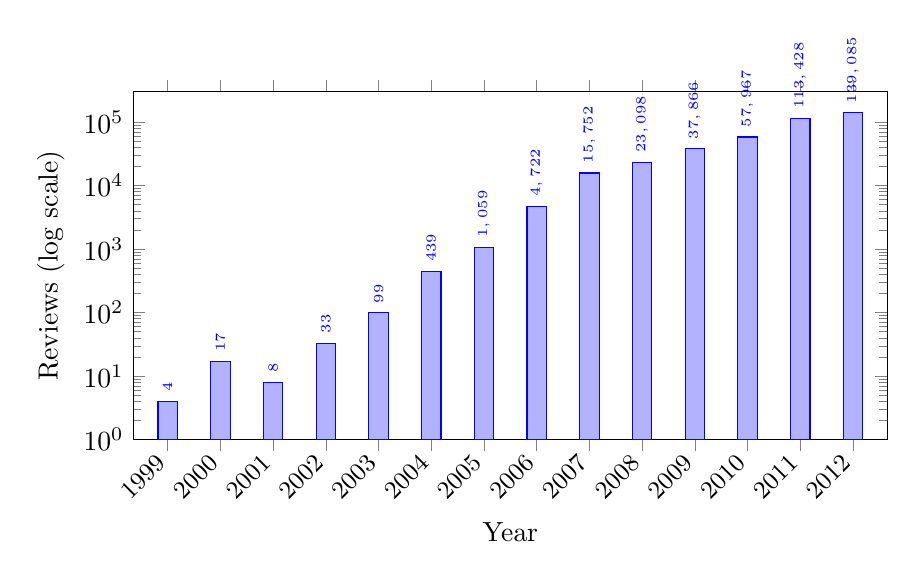
\begin{tikzpicture}
\begin{axis}[
  ybar, ymode=log, ymin=1, ymax=300000,
  width=0.92\textwidth, height=6cm,
  bar width=7pt,
  xlabel={Year}, ylabel={Reviews (log scale)},
  symbolic x coords={1999,2000,2001,2002,2003,2004,2005,2006,2007,2008,2009,2010,2011,2012},
  xtick=data, x tick label style={rotate=45,anchor=east,font=\small},
  point meta=explicit,
  nodes near coords={\pgfmathprintnumber[fixed,precision=0,1000 sep={,}]{\pgfplotspointmeta}},
  nodes near coords style={font=\tiny,rotate=90,anchor=west},
  enlarge x limits=0.05
]
\addplot coordinates {(1999,4) [4] (2000,17) [17] (2001,8) [8] (2002,33) [33] (2003,99) [99] (2004,439) [439] (2005,1059) [1059] (2006,4722) [4722] (2007,15752) [15752] (2008,23098) [23098] (2009,37866) [37866] (2010,57967) [57967] (2011,113428) [113428] (2012,139085) [139085]};
\end{axis}
\end{tikzpicture}
\end{center}

The number of cleaned reviews grows roughly exponentially from 2006, and 2011--2012 together hold 252{,}513 reviews (64.2\%); 2012 ends in October. The mean star rating drifts down from 4.386 in 2007 to 4.112 in 2012, and the negative share rises from 10.0\% to 16.1\%. The label distribution is therefore not stable in time.

The split in Section~\ref{sec:5-5} is random, so training and test reviews come from the same period. This does not measure how a model would fare on future reviews, and is listed as a limitation.

\section{Users, Products and Helpfulness}
\label{sec:4-6}

There are 256{,}044 distinct users and 67{,}554 distinct products. Of the users, 80.3\% wrote a single review, and 78.7\% of the products have five reviews or fewer. Both distributions have a long tail, so a model cannot rely on a user's rating habits and has to learn from the text.

Among reviews with at least five votes, negative reviews attract more votes but a lower helpful ratio, because readers often disagree with a complaint. Since this information is not available when a review is posted, it is not used as a feature (Section~\ref{sec:3-5}).

\section{Noise in the Text}
\label{sec:4-7}

\begin{center}
\begin{tabular}{@{}p{8cm}p{3cm}@{}}
    \toprule
    Noise in \texttt{Text} & Share of reviews \\
    \midrule
    HTML tags (mostly \texttt{<br />}) & 26.14\% \\
    URLs (\texttt{http}, \texttt{www}) & 2.08\% \\
    Encoded HTML characters (\texttt{\&amp;}, \texttt{\&quot;}) & 0.33\% \\
    \bottomrule
\end{tabular}
\end{center}

The text is therefore cleaned lightly (Section~\ref{sec:5-3}). Stop words and punctuation are \emph{kept}, because negations such as \emph{not}, \emph{no} and \emph{never} appear in standard stop-word lists but decide the sentiment, and because the neural models can learn the role of each word from context.

\section{Vocabulary of Each Class}
\label{sec:4-8}

Counting words and word pairs on a class-balanced sample of 20{,}000 reviews per class (stop words removed except negations) shows that single words such as \emph{like}, \emph{taste}, \emph{good} and \emph{coffee} occur in all three classes; \emph{good} is frequent even in negative reviews (``not good'', ``good but\ldots''). Word pairs separate the classes better: \emph{highly recommend}, \emph{great product} and \emph{love this} in positive reviews; \emph{waste money}, \emph{would not} and \emph{not buy} in negative ones. The neutral class has no vocabulary of its own and mixes that of the other two, so it is expected to be the hardest class.

\section{Design Decisions for Data Preparation}
\label{sec:4-9}

\begin{center}
\begin{tabular}{@{}p{6.2cm}p{7.9cm}@{}}
    \toprule
    Finding & Decision \\
    \midrule
    About 31\% of raw rows are repeated reviews & Remove them before splitting \\
    Labels skewed 77.9 / 14.5 / 7.6\% & Stratified split; class weights in the loss; Macro-F1 as main metric \\
    Right-skewed length; 200 words $\approx$ 93\% coverage & Limit of 200 words (BiLSTM) and 256 tokens (Transformer); dynamic padding and bucketing \\
    Titles are short but informative & Input is title followed by body \\
    26\% of bodies contain HTML & Light cleaning; keep punctuation and negations \\
    Context and negation matter & Use a sequence model (BiLSTM with attention) and a Transformer \\
    Label distribution drifts over time & Report as a limitation; the split is random \\
    \bottomrule
\end{tabular}
\end{center}


\chapter{Data Preparation}
\label{ch:data-preparation}
\section{Objective}
\label{sec:5-1}

Turn the raw reviews into a leakage-safe modelling dataset: clean the raw rows (Section~\ref{sec:5-2}), build the input text (Section~\ref{sec:5-3}) and the label (Section~\ref{sec:5-4}), split the reviews into three parts (Section~\ref{sec:5-5}) and compute class weights (Section~\ref{sec:5-7}). The chapter implements the design decisions of Section~\ref{sec:4-9} with one frozen configuration:

\begin{center}
\begin{tabular}{@{}p{5.2cm}p{3cm}p{5.8cm}@{}}
    \toprule
    Parameter & Value & Origin \\
    \midrule
    Split ratio train / val / test & 80 / 10 / 10\% & Large test part; validation for early stopping \\
    Stratification & By label & Neutral is only 7.6\% (Section~\ref{sec:4-3}) \\
    Random seed & 42 & Reproducible split \\
    Sequence limit & 200 words / 256 tokens & Length coverage (Section~\ref{sec:4-4}) \\
    \bottomrule
\end{tabular}
\end{center}

\section{Data Cleaning}
\label{sec:5-2}

Each data-quality issue is first measured on the full raw file of 568{,}454 rows (rows may overlap across rules):

\begin{center}
\begin{tabular}{@{}p{7cm}p{3cm}p{3cm}@{}}
    \toprule
    Issue & Rows & Share of rows \\
    \midrule
    Repeated review (same user, name, time, text) & 174{,}521 & 30.70\% \\
    Repeated \texttt{Text} & 174{,}875 & 30.76\% \\
    Missing \texttt{Summary} & 27 & 0.005\% \\
    Missing \texttt{ProfileName} & 26 & 0.005\% \\
    Numerator $>$ denominator (helpfulness) & 2 & $<$0.001\% \\
    \bottomrule
\end{tabular}
\end{center}

No row is duplicated in \emph{all} columns, so the repetition is hidden in the product code. For example, user \texttt{A395BORC6FGVXV} posted one 2-star review titled ``Cough Medicine'' at time 1307923200, and it appears three times under three different product codes (\texttt{B000UA0QIQ}, \texttt{B002Y7526Y}, \texttt{B000U9WZ54}). Left in, such copies would put one on each side of a random split.

The cleaning is performed in this order, always keeping the first occurrence:
\begin{enumerate}
    \item Drop rows that repeat the key (\texttt{UserId}, \texttt{ProfileName}, \texttt{Time}, \texttt{Text}).
    \item Drop rows with \texttt{HelpfulnessNumerator} $>$ \texttt{HelpfulnessDenominator}, which is impossible by definition.
    \item Drop rows whose \texttt{Text} is still identical to an earlier row's (copies between accounts, spam).
    \item Replace a missing \texttt{Summary} by an empty string and create the label from \texttt{Score} (Section~\ref{sec:5-4}).
\end{enumerate}

\begin{center}
\begin{tabular}{@{}p{7cm}p{3cm}p{3cm}@{}}
    \toprule
    Stage & Rows left & Rows removed \\
    \midrule
    Raw file & 568{,}454 & -- \\
    After step 1 (repeated key) & 393{,}933 & 174{,}521 \\
    After step 2 (invalid helpfulness) & 393{,}931 & 2 \\
    After step 3 (repeated \texttt{Text}) & 393{,}577 & 354 \\
    \bottomrule
\end{tabular}
\end{center}

\textbf{Result.} Cleaning removes 174{,}877 rows (30.8\% of 568{,}454) and leaves \textbf{393{,}577 reviews}. Step 3 keeps the first occurrence regardless of its star rating. It also removes legitimate but identical short reviews written by different people, which is a deliberate trade: it costs 354 rows (0.09\% of the data) and closes the remaining leakage route. The cleaned table is saved once and read by every later stage.

\section{Building the Model Input Text}
\label{sec:5-3}

The model input is
\begin{equation*}
    \text{text} = \operatorname{clean}(\texttt{Summary}) + \text{``. ''} + \operatorname{clean}(\texttt{Text}),
\end{equation*}
where $\operatorname{clean}$ unescapes HTML entities, deletes HTML tags and URLs, and collapses whitespace. It does not lowercase, remove punctuation or remove stop words (Section~\ref{sec:4-7}). The separator follows three rules:
\begin{itemize}
    \item If the title is non-empty and does not end with ``.'', ``!'' or ``?'', the two parts are joined with ``. ''.
    \item If the title already ends with one of those marks, the parts are joined with a single space.
    \item If the title is empty (27 raw rows have a missing title), the input is the cleaned body alone.
\end{itemize}
For example, the review titled ``Not as Advertised'' becomes ``Not as Advertised. Product arrived labeled as Jumbo Salted Peanuts\ldots'', and the body fragment ``\ldots were bummed.\texttt{<br />}\texttt{<br />}Now, because\ldots'' becomes ``\ldots were bummed. Now, because\ldots''. Cleaning all 393{,}577 reviews took 19.5 seconds. Tokenisation depends on the model (a word vocabulary for the BiLSTM, WordPiece for the Transformer), so it is done in the modelling chapters.

\section{Label Construction}
\label{sec:5-4}

The label is derived from \texttt{Score} with the mapping of Section~\ref{sec:2-2}: 1 and 2 stars give negative (0), 3 stars neutral (1), 4 and 5 stars positive (2).

\section{Train, Validation and Test Split}
\label{sec:5-5}

The data are split in two stratified stages with a fixed seed: 80\% for training and 20\% held out, then the held-out part is divided equally into validation and test.

\begin{lstlisting}
train_df, temp_df = train_test_split(
    df[cols], test_size=0.2, stratify=df['label'], random_state=SEED)
val_df, test_df = train_test_split(
    temp_df, test_size=0.5, stratify=temp_df['label'], random_state=SEED)
\end{lstlisting}

\begin{center}
\begin{tabular}{@{}lrrrr@{}}
    \toprule
    Part & Reviews & negative & neutral & positive \\
    \midrule
    Train & 314{,}861 & 45{,}654 & 23{,}803 & 245{,}404 \\
    Validation & 39{,}358 & \multicolumn{3}{c}{same proportions as train} \\
    Test & 39{,}358 & \multicolumn{3}{c}{same proportions as train} \\
    \bottomrule
\end{tabular}
\end{center}

The proportions are about 14.5\%, 7.6\% and 77.9\% in every part because the split is stratified. Training updates the weights. Validation drives early stopping, the choice of the best epoch and the later calibration of the neutral threshold. Test is used once, at the end, for the reported results. Because the seed and the rule are fixed, a re-run produces the same three parts.

\section{Class Weights}
\label{sec:5-7}

Let $N$ be the number of training reviews, $K=3$ the number of classes and $N_c$ the number of training reviews of class $c$. The weight of class $c$ is
\begin{equation*}
    w_c = \frac{N}{K\,N_c},
\end{equation*}
and the loss over a batch is
\begin{equation*}
    \mathcal{L} = -\frac{1}{\sum_i w_{y_i}} \sum_i w_{y_i}\log \hat p_{i,y_i}.
\end{equation*}
A rare class receives a large weight, so an error on it costs more and its gradient is not drowned by the majority class. The weights are computed from the training counts only:

\begin{center}
\begin{tabular}{@{}lrr@{}}
    \toprule
    Class & Training reviews $N_c$ & Weight $w_c$ \\
    \midrule
    negative & 45{,}654 & 2.299 \\
    neutral & 23{,}803 & 4.409 \\
    positive & 245{,}404 & 0.428 \\
    \bottomrule
\end{tabular}
\end{center}

A neutral review weighs about 10 times as much as a positive one ($4.409/0.428 \approx 10.3$), which is exactly the imbalance ratio of Section~\ref{sec:4-3}.

\section{Leakage Prevention and Random Split}
\label{sec:5-8}

\begin{itemize}
    \item \textbf{Repeated text.} Duplicates are removed \emph{before} the split (Section~\ref{sec:5-2}), so the same text cannot sit in both training and test.
    \item \textbf{Statistics from training only.} Class weights are computed from the training part (Section~\ref{sec:5-7}); the BiLSTM word vocabulary is built from the training part only (modelling chapter).
    \item \textbf{Test used once.} Epoch choice and the neutral threshold are tuned on validation; test is read for the final report.
    \item \textbf{Random, not chronological.} Training and test reviews come from the same period, although the label distribution drifts (Section~\ref{sec:4-5}). The scores therefore do not measure performance on future reviews.
    \item \textbf{No automatic check.} The class proportions of each part are printed and compared by eye; there is no assertion, so a change to the split code should be re-checked against the table of Section~\ref{sec:5-5}.
\end{itemize}

\section{Conclusion}
\label{sec:5-9}

The raw 568{,}454 reviews become 393{,}577 cleaned reviews, split into 314{,}861 training, 39{,}358 validation and 39{,}358 test reviews, with class weights of 2.299, 4.409 and 0.428 for negative, neutral and positive. The next chapters train the models on the training part, select on validation and report on test.


\chapter{Modeling}
\label{ch:modeling}
\section{Objective}
\label{sec:6-1}

Train two neural networks on the same training part and score them, together with the rule ``always answer positive'', on the same test reviews (Chapter~\ref{ch:data-preparation}): a BiLSTM with attention trained from scratch (Section~\ref{sec:6-3}), and a BERT encoder fine-tuned on the data (Section~\ref{sec:6-5}). The always-positive rule is a reference that is not trained. Section~\ref{sec:6-bg} first explains what LSTM, BiLSTM, attention and BERT are and why they are used.

Both networks use the class-weighted cross-entropy of Section~\ref{sec:5-7}, select their settings on the validation part only, and read the test part once. Every number in this chapter comes from the training and validation runs; test results are in Chapter~\ref{ch:evaluation}.

\section{Background: Why Sequence Models and Transformers}
\label{sec:6-bg}

This section introduces, at the depth the later sections need, the concepts behind the two neural models and the reason each is used here.

\subsection*{Why the order of words matters}

A model that only counts words and word pairs cannot tell ``not good'' from ``good'' once the negation is two or more words away (``not really all that good''), and it cannot tell who is praised in ``the coffee was fine but the delivery was awful''. Section~\ref{sec:4-8} showed that single words such as \emph{good} occur in all three classes, and that pairs separate the classes better. A model that reads the review \emph{in order} and carries information from earlier words to later ones can use this context. Two families of such models are used.

\subsection*{Recurrent networks and the LSTM}

A recurrent network reads the words one at a time and keeps a hidden state $h_t$ that summarises everything read so far. A plain recurrent network loses information over long texts, because the gradient that trains it shrinks at every step (the \emph{vanishing gradient} problem). The \textbf{Long Short-Term Memory} (LSTM) unit fixes this with a memory cell $c_t$ and three gates, which decide what to forget, what to write and what to output:
\begin{align*}
    f_t &= \sigma(W_f[h_{t-1},x_t]+b_f), & i_t &= \sigma(W_i[h_{t-1},x_t]+b_i),\\
    o_t &= \sigma(W_o[h_{t-1},x_t]+b_o), & c_t &= f_t\odot c_{t-1} + i_t\odot\tanh(W_c[h_{t-1},x_t]+b_c),\\
    h_t &= o_t\odot\tanh(c_t), & &
\end{align*}
where $x_t$ is the vector of the $t$-th word and $\sigma$ is the logistic function. The cell $c_t$ is changed only by addition and element-wise gating, so information, and gradient, can travel across many words. An LSTM therefore suits reviews of tens to hundreds of words.

\subsection*{Why bidirectional, and why attention}

A one-directional LSTM reads left to right, so its state at a word knows only the words before it. A \textbf{bidirectional LSTM} (BiLSTM) runs a second LSTM from right to left and joins the two states, $h_t=[\overrightarrow{h_t};\overleftarrow{h_t}]$. The state at each word then depends on the words on both sides, which helps when the meaning of a word is set by what follows it (``\emph{good} \ldots{} but not worth the price'').

The sentiment of a review is not carried equally by every word. \textbf{Attention pooling} learns a weight $\alpha_t$ for each position and forms the review vector as the weighted sum of the states (equations in Section~\ref{sec:6-3}), instead of keeping only the last state, where early words are weakest. The weights can also be shown on the text, which makes the model inspectable.

BiLSTM with attention was chosen because it is a standard, small sequence model for sentiment that can be trained from scratch on this data in minutes, it reads context in both directions, and it is inspectable.

\subsection*{The Transformer and BERT}

A recurrent network passes information from word to word, so a distant pair of words is linked only through many steps. The \textbf{Transformer} replaces this with \emph{self-attention}: every token compares itself directly with every other token of the review,
\begin{equation*}
    \text{Attention}(Q,K,V)=\operatorname{softmax}\!\left(\frac{QK^\top}{\sqrt{d_k}}\right)V,
\end{equation*}
where the queries $Q$, keys $K$ and values $V$ are linear maps of the token vectors. Several such \emph{heads} work in parallel, and a vector for the position of each token is added because self-attention alone ignores order. A stack of such layers is an \emph{encoder}.

\textbf{BERT} (Bidirectional Encoder Representations from Transformers) is a Transformer encoder that was first \emph{pre-trained}, by its authors, on a very large amount of English text (Wikipedia and BookCorpus) without any sentiment labels. Its task was to predict words hidden in the text (masked language modelling) and whether one sentence follows another. This teaches the network the grammar, the meaning of words in context and common negation patterns. Text is split into WordPiece sub-words, so a rare word becomes known pieces (\emph{unbelievable} $\to$ \emph{un}, \emph{\#\#bel}, \emph{\#\#ie}, \ldots) and no word is unknown. The first token of every input is a special \texttt{[CLS]} token whose final vector represents the whole text.

\textbf{Fine-tuning} is \emph{transfer learning}: a small output layer for the three classes is added on top of the \texttt{[CLS]} vector, and the whole pre-trained network is trained a little further on the labelled reviews, with a small learning rate so that the learned knowledge is adjusted, not erased. In contrast to the BiLSTM, which learns language from the 315{,}000 training reviews alone, BERT starts with the knowledge of billions of words, and the project tests how much this helps. \texttt{bert-base-uncased} is the smaller of the two original sizes (12 layers, 109 million parameters) and lower-cases the text, which keeps the setup simple.

\section{BiLSTM with Attention}
\label{sec:6-3}

\subsection*{Input}

The input text of Section~\ref{sec:5-3} is lower-cased and split by a regular expression that keeps contractions (\emph{don't}) and the marks \texttt{!} and \texttt{?}. The vocabulary holds the words that occur at least three times in the training part, capped at 50{,}000; it ends with 46{,}760 entries, including the padding and unknown symbols. It covers 99.71\% of the training tokens. Each review is cut at 200 words, which cuts 6.47\% of the training reviews. Batches of 256 reviews are formed by length bucketing: the data are shuffled, grouped into chunks, sorted by length inside each chunk and cut into batches, so that reviews of similar length share a batch and padding is small. There are 1{,}230 batches per epoch.

\subsection*{Architecture}

\begin{center}
\begin{tabular}{@{}p{3.6cm}p{10.4cm}@{}}
    \toprule
    Layer & Role \\
    \midrule
    Embedding $46{,}760\times128$ & a trainable vector per word, dropout 0.3 \\
    BiLSTM, 128 units per direction & reads the review left-to-right and right-to-left; the state at position $t$ is $h_t\in\mathbb{R}^{256}$ \\
    Attention pooling & weights each position and sums the states \\
    Dropout 0.3, Linear $256\to3$ & class scores \\
    \bottomrule
\end{tabular}
\end{center}

The attention layer scores each state, normalises the scores over the real (non-padding) positions, and uses the weighted sum as the review vector:
\begin{equation*}
    e_t = \mathbf{w}^\top h_t,\qquad
    \alpha_t = \frac{\exp(e_t)}{\sum_k \exp(e_k)},\qquad
    \mathbf{c} = \sum_t \alpha_t h_t .
\end{equation*}
Padding positions get a score of $-10^{9}$ before the softmax, so their weight is zero. The model has 6{,}250{,}500 trainable parameters, of which 5{,}985{,}280 are the embedding.

\subsection*{Training}

\begin{center}
\begin{tabular}{@{}p{5cm}p{9cm}@{}}
    \toprule
    Setting & Value \\
    \midrule
    Optimiser & AdamW, learning rate $2\times10^{-3}$, weight decay $10^{-4}$ \\
    Schedule & learning rate halved when validation Macro-F1 does not improve \\
    Gradient clipping & norm 1.0 \\
    Epochs, early stopping & at most 5; stop after 2 epochs without improvement; keep the best epoch \\
    Seed & 42 \\
    \bottomrule
\end{tabular}
\end{center}

The run used all 5 epochs; the best validation Macro-F1 is 0.7504 at epoch 4, and the model of that epoch is kept. Training takes 3.4 minutes on one Tesla T4 GPU.

\begin{center}
\small
\begin{tabular}{@{}rrrrrr@{}}
    \toprule
    Epoch & Train loss & Validation loss & Validation accuracy & Validation Macro-F1 & Learning rate \\
    \midrule
    1 & 0.6168 & 0.5283 & 0.8646 & 0.7275 & 0.002 \\
    2 & 0.4956 & 0.5292 & 0.8830 & 0.7469 & 0.002 \\
    3 & 0.4549 & 0.5049 & 0.8614 & 0.7318 & 0.002 \\
    4 & 0.4100 & 0.5376 & 0.8820 & \textbf{0.7504} & 0.001 \\
    5 & 0.3894 & 0.5342 & 0.8772 & 0.7469 & 0.001 \\
    \bottomrule
\end{tabular}
\end{center}

The training loss falls steadily while the validation loss stays near 0.53 and is lowest at epoch 3, which signals overfitting from about epoch 3 or 4. The epoch is chosen by Macro-F1, not by validation loss, and the differences between the last epochs (about 0.003) are small.

\section{Fine-tuning BERT}
\label{sec:6-5}

\texttt{bert-base-uncased} is a 12-layer Transformer encoder (hidden size 768, 12 attention heads) pre-trained on Wikipedia and BookCorpus. A new three-class layer is placed on the representation of the \texttt{[CLS]} token and the whole network is trained. The configuration is a single run without hyperparameter search.

\begin{center}
\begin{tabular}{@{}p{5cm}p{9cm}@{}}
    \toprule
    Setting & Value \\
    \midrule
    Tokenisation & WordPiece, cut at 256 tokens; dynamic padding with length bucketing \\
    Truncation & about 6.2\% of reviews (measured on 3{,}000 training reviews; median length 80, 90th percentile 207 tokens) \\
    Batch, epochs & 32 reviews, 2 epochs; 9{,}840 steps per epoch, 19{,}680 in total \\
    Optimiser & AdamW, learning rate $3\times10^{-5}$, weight decay 0.01 (not applied to biases and LayerNorm) \\
    Schedule & linear warm-up over the first 10\% of steps, then linear decay to 0 \\
    Other & fp16 mixed precision, gradient clipping 1.0, seed 42 \\
    Parameters & 109{,}484{,}547 \\
    \bottomrule
\end{tabular}
\end{center}

After each epoch the model is scored on the validation part and saved if its Macro-F1 is the best so far; there is no early stopping. Each epoch takes 32.2 minutes on a Tesla T4, 64.4 minutes in total.

\begin{center}
\begin{tabular}{@{}rrrr@{}}
    \toprule
    Epoch & Train loss & Validation accuracy & Validation Macro-F1 \\
    \midrule
    1 & 0.4943 & 0.8884 & 0.7664 \\
    2 & 0.3517 & 0.9069 & \textbf{0.7864} \\
    \bottomrule
\end{tabular}
\end{center}

Validation Macro-F1 is still rising at the last epoch, so the model has not saturated and more epochs might help; with two epochs overfitting cannot be observed.

\section{Summary of the Models}
\label{sec:6-7}

\begin{center}
\small
\begin{tabular}{@{}p{3.6cm}p{3.4cm}rp{3.6cm}@{}}
    \toprule
    Model & Trained on this data & Parameters & Selection on validation \\
    \midrule
    BiLSTM + attention & yes, from scratch & 6.25 M & epoch, early stopping \\
    BERT-base & yes, fine-tuned & 109.48 M & epoch \\
    Always positive & no & 0 & -- \\
    \bottomrule
\end{tabular}
\end{center}

Both networks were trained on one Tesla T4 GPU, so their training times are comparable.


\chapter{Evaluation}
\label{ch:evaluation}
\section{Objective}
\label{sec:7-1}

Measure how well each model assigns sentiment to reviews it has not seen, compare the two networks fairly, and find where they fail. The protocol is fixed before the results: Macro-F1 (Section~\ref{sec:2-4}) is the main metric; the test part of 39{,}358 reviews is read once; every choice (epoch, neutral threshold) is made on the validation part. Confidence intervals come from 1{,}000 bootstrap resamples of the test reviews, with all models scored on the same resample so that differences can be paired. The intervals reflect the sampling error of the test part only, not the choice of random seed.

\section{Results on the Full Test Part}
\label{sec:7-2}

\begin{center}
\small
\begin{tabular}{@{}lrrrrrr@{}}
    \toprule
    Model & Accuracy & Macro-F1 & \shortstack[r]{F1\\negative} & \shortstack[r]{F1\\neutral} & \shortstack[r]{F1\\positive} & \shortstack[r]{Macro-F1\\95\% interval} \\
    \midrule
    BERT-base fine-tuned & \textbf{0.9074} & \textbf{0.7877} & \textbf{0.8470} & \textbf{0.5540} & \textbf{0.9620} & [0.7814, 0.7929] \\
    BiLSTM + attention & 0.8788 & 0.7422 & 0.7863 & 0.4916 & 0.9488 & [0.7360, 0.7480] \\
    Always positive & 0.7794 & 0.2920 & 0 & 0 & 0.8760 & [0.2911, 0.2929] \\
    \bottomrule
\end{tabular}
\end{center}

\begin{center}
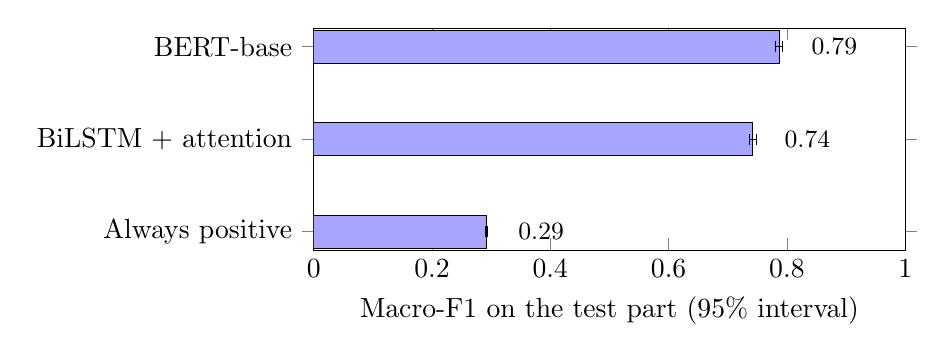
\begin{tikzpicture}
\begin{axis}[
  xbar, xmin=0, xmax=1, width=0.75\textwidth, height=4.4cm,
  symbolic y coords={Always positive,BiLSTM + attention,BERT-base},
  ytick=data, xlabel={Macro-F1 on the test part (95\% interval)},
  bar width=12pt, nodes near coords, nodes near coords align={horizontal},
  every node near coord/.append style={font=\small, xshift=8pt}
]
\addplot[fill=blue!35, error bars/.cd, x dir=both, x explicit] coordinates {
  (0.2920,Always positive) += (0.0009,0) -= (0.0009,0)
  (0.7422,BiLSTM + attention) += (0.0058,0) -= (0.0062,0)
  (0.7877,BERT-base) += (0.0052,0) -= (0.0063,0)
};
\end{axis}
\end{tikzpicture}
\end{center}

Both networks are far above the always-positive rule (Macro-F1 0.292, which scores 0.78 accuracy while recognising nothing about the other two classes). BERT is best on every column. The F1 of the neutral class is the lowest for both networks, 0.49 and 0.55.

\textbf{Cost.} Both networks were trained and timed on a Tesla T4.

\begin{center}
\small
\begin{tabular}{@{}lrrr@{}}
    \toprule
    Model & Training time & Inference on the test part & Parameters \\
    \midrule
    BERT-base & 64.4 min & 83.7 s & 109.48 M \\
    BiLSTM + attention & 3.4 min & 3.7 s & 6.25 M \\
    \bottomrule
\end{tabular}
\end{center}

BERT needs about 19 times the training time, 23 times the inference time and 17.5 times the parameters of the BiLSTM for 0.0455 more Macro-F1. The BiLSTM reaches about 94\% of the Macro-F1 of BERT with about 5\% of its training time.

\section{Is the Neutral Class the Problem?}
\label{sec:7-3}

Both networks have high recall but low precision on neutral: they predict neutral for too many reviews. The table gives, for each model, the share of true neutral reviews that are predicted correctly, and the true label of the reviews it predicts as neutral.

\begin{center}
\small
\begin{tabular}{@{}lrrrrrr@{}}
    \toprule
     & \multicolumn{3}{c}{True neutral predicted as} & \multicolumn{3}{c}{Predicted neutral are truly} \\
    \cmidrule(lr){2-4}\cmidrule(lr){5-7}
    Model & negative & neutral & positive & negative & neutral & positive \\
    \midrule
    BERT-base & 19.7\% & 68.1\% & 12.1\% & 17.9\% & 46.7\% & 35.4\% \\
    BiLSTM + attention & 16.5\% & 67.6\% & 15.9\% & 23.4\% & 38.6\% & 38.0\% \\
    \bottomrule
\end{tabular}
\end{center}

Both networks recover about two thirds of the neutral reviews, but fewer than half of the reviews they call neutral are neutral. The cause is partly the data (a 3-star review often praises and complains at once, and the neutral class has no vocabulary of its own, Section~\ref{sec:4-8}) and partly the loss, whose neutral weight is 4.4 times a typical weight (Section~\ref{sec:5-7}).

\section{Performance by Review Length}
\label{sec:7-5}

\begin{center}
\small
\begin{tabular}{@{}lrrrrrr@{}}
    \toprule
    Words per review & $\le$30 & 31--60 & 61--100 & 101--200 & 201--400 & $>$400 \\
    Reviews in the test part & 6{,}137 & 13{,}659 & 9{,}601 & 7{,}534 & 2{,}100 & 327 \\
    \midrule
    BERT-base & 0.778 & 0.783 & 0.794 & 0.796 & 0.758 & 0.693 \\
    BiLSTM + attention & 0.753 & 0.738 & 0.746 & 0.747 & 0.704 & 0.600 \\
    \bottomrule
\end{tabular}
\end{center}

Both models are lowest on reviews longer than 400 words, and the BiLSTM drops the most (0.600 against 0.693 for BERT). The BiLSTM keeps only the first 200 words and BERT the first 256 tokens, so both lose the end of a long review. The last group has only 327 reviews, so its scores vary more and should not be over-read.

\section{Bootstrap Interval for the Difference}
\label{sec:7-6}

The difference in Macro-F1 between BERT and the BiLSTM on the full test part is $+0.0454$, with a 95\% interval of $[+0.0400,\,+0.0507]$ over the paired bootstrap resamples. The interval does not contain zero, so the difference is larger than the sampling error of the test part, and BERT is ahead of the BiLSTM in 100\% of the resamples.

\section{Calibrating the Neutral Threshold}
\label{sec:7-7}

Because the models over-predict neutral, a constant \texttt{bias} is added to the log-probability of neutral before taking the arg\,max (a negative bias predicts neutral less often). The bias is chosen on the validation part to maximise Macro-F1 and then applied once to the test part. This needs no retraining.

\begin{center}
\small
\begin{tabular}{@{}lrrrr@{}}
    \toprule
    Model & \shortstack[r]{Chosen\\bias} & \shortstack[r]{Validation Macro-F1\\before $\to$ after} & \shortstack[r]{Test Macro-F1\\before $\to$ after} & \shortstack[r]{Test F1 neutral\\before $\to$ after} \\
    \midrule
    BiLSTM + attention & $-0.8$ & 0.7504 $\to$ 0.7577 & 0.7422 $\to$ 0.7551 & 0.4916 $\to$ 0.4978 \\
    BERT-base & $-1.1$ & 0.7864 $\to$ 0.7902 & 0.7877 $\to$ 0.7866 & 0.5540 $\to$ 0.5448 \\
    \bottomrule
\end{tabular}
\end{center}

The adjustment helps the BiLSTM (+0.013 on the test part) but not BERT: the gain of 0.004 that BERT shows on validation does not carry over to the test part and lies within the noise. The headline results of this report use no bias (Section~\ref{sec:7-2}); the calibration is an extra experiment.

\section{Error Analysis and Examples}
\label{sec:7-8}

\subsection*{Confident errors of the best model}

BERT predicts \emph{negative} for 165 reviews of 5 stars and \emph{positive} for 58 reviews of 1 star; 948 neutral reviews are misclassified. Many confident errors look like noisy labels: the author gave 5 stars but wrote a complaint (``Now I would not recommend it to my worst enemy. The coffee now has no aroma\ldots'', ``Incredibly overpriced\ldots this is a total and complete rip off''), or 1 star with praise (``LOVE LOVE LOVE THESE! (edited because NO longer available in prime)''). In these cases the model reads the text better than the star count does. Not every case is noise: ``My dogs won't eat anything else. My dogs will not eat anything but the Iams biscuit'' praises the product, and the model misreads it. The share of noisy labels among the errors was not counted, so this report does not give a rate.

A related property of the data: about 3.4\% of test reviews (1{,}350) contain a phrase such as ``3 stars'', and only about 59\% of them state the true rating (the others read ``5 star service'' or ``4 stars out of 5''). These texts are kept, so some signal flows from the label into the text for both models.

\subsection*{Sentences written for the test}

Six sentences written by the authors give a qualitative check; they are not a substitute for the measurements above.

\begin{center}
\small
\begin{tabular}{@{}p{7.2cm}ll@{}}
    \toprule
    Sentence & BiLSTM & BERT \\
    \midrule
    ``This coffee is absolutely amazing, I will definitely buy it again!'' & pos (100\%) & pos (100\%) \\
    ``Not bad at all, actually pretty tasty.'' & neu (78\%) & pos (79\%) \\
    ``It's okay. Nothing special, but it does the job.'' & neu (100\%) & neu (99\%) \\
    ``Great, another box arrived completely crushed. Just what I needed.'' & pos (87\%) & pos (99\%) \\
    ``My dog loves these treats, but they are way too expensive for such a small bag.'' & neu (84\%) & neu (89\%) \\
    ``I would not recommend this to anyone. Total waste of money.'' & neg (100\%) & neg (100\%) \\
    \bottomrule
\end{tabular}
\end{center}

Both models read the sarcastic fourth sentence as positive, because ``great'' and ``just what I needed'' sound positive. Both label the mixed third and fifth sentences neutral, and the clearly positive and negative sentences correctly. For the second sentence the BiLSTM answers neutral and BERT positive; both are acceptable for such mild praise. The attention weights of the BiLSTM mostly fall on words that carry sentiment or reverse it (\emph{mistake}, \emph{great}, \emph{not}, \emph{okay}, \emph{but}), but not always: for one neutral review the largest weight is on a product name (\emph{stevia}). Attention shows where the model looks, not a complete explanation.

\section{Limitations}
\label{sec:7-9}

\begin{itemize}
    \item \textbf{Weak labels.} Stars do not always match the text (Section~\ref{sec:7-8}), and the 3-star boundary is subjective, which bounds the quality any model can show.
    \item \textbf{Sarcasm and mixed opinions.} Both models fail on sarcasm, and neutral stays the hardest class (F1 0.49 and 0.55).
    \item \textbf{Random split.} The label distribution drifts over time (Section~\ref{sec:4-5}) and the same user or product can sit in both training and test, so the scores do not measure performance on future reviews.
    \item \textbf{Runs and seeds.} Each model was trained once (seed 42), so the bootstrap intervals do not cover variation between seeds.
    \item \textbf{BERT is not saturated.} It was fine-tuned for 2 epochs with one fixed configuration, so its score may be a lower bound.
    \item \textbf{Different truncation.} The BiLSTM keeps 200 words and BERT 256 tokens.
    \item \textbf{One domain.} All data are English food reviews from Amazon, 1999--2012.
\end{itemize}


\chapter{Conclusion}
\label{ch:conclusion}
\section{Summary}
\label{sec:8-1}

The project turned 568{,}454 Amazon food reviews into a leakage-safe corpus of 393{,}577 cleaned reviews (Chapter~\ref{ch:data-preparation}), split 80/10/10 with stratification, and compared two trained classifiers with the always-positive rule on a three-class sentiment task labelled from star ratings.

\begin{itemize}
    \item \textbf{Fine-tuned BERT-base is the better model:} Macro-F1 0.7877 and accuracy 0.9074 on the 39{,}358 test reviews, ahead of the BiLSTM with attention (0.7422) by 0.0455, with a 95\% interval of $[+0.0400,\,+0.0507]$ for the difference. It is ahead on all three classes, so transfer learning beats learning from scratch on this task.
    \item \textbf{Neutral is the weak point of both models} (F1 0.49 and 0.55): they predict it too often, and shifting the threshold helps only the BiLSTM.
    \item \textbf{Cost.} BERT needs 19 times the training time and 17.5 times the parameters of the BiLSTM for 0.0455 more Macro-F1.
\end{itemize}

\section{Limitations}
\label{sec:8-2}

The limits are listed with their measurements in Section~\ref{sec:7-9}. The most important are: star labels that do not always match the text; a random split that does not measure performance on future reviews; a single run for each model; and a BERT model that was fine-tuned for only two epochs, with validation Macro-F1 still rising.

\section{Future Work}
\label{sec:8-3}

\begin{enumerate}
    \item \textbf{Longer or repeated fine-tuning of BERT} (more epochs, several seeds), and stronger encoders such as RoBERTa-base or DeBERTa-v3, to test whether the BERT score is a lower bound.
    \item \textbf{A time-based split} (train until 2011, test on 2012) to measure performance on later reviews and the effect of the drift of the label distribution.
    \item \textbf{Pre-trained word vectors} (GloVe, fastText) for the BiLSTM embedding, to see whether the gap to BERT narrows.
    \item \textbf{Other ways to treat the imbalance} (focal loss, oversampling), because the large neutral weight may cause the over-prediction of neutral.
    \item \textbf{Head-and-tail truncation} for long reviews, where both models scored lowest.
    \item \textbf{A small human-labelled sample}, not based on stars, to measure how much of the error is label noise.
\end{enumerate}

\section{Reproducibility}
\label{sec:8-4}

The split uses a fixed seed and rule and all predictions on the test part are stored, so every table of Chapter~\ref{ch:evaluation} can be recomputed from them. The code is one notebook (cleaning, understanding and preparation of the data, BiLSTM, BERT and evaluation) and a shared package \texttt{src/}.


\begin{thebibliography}{9}
\bibitem{mcauley2013} J.~McAuley and J.~Leskovec. From amateurs to connoisseurs: modeling the evolution of user expertise through online reviews. In \emph{Proceedings of the 22nd International Conference on World Wide Web (WWW)}, 2013.
\bibitem{kaggle_fine_food} Stanford Network Analysis Project. Amazon Fine Food Reviews (Kaggle dataset \texttt{snap/amazon-fine-food-reviews}). \url{https://www.kaggle.com/datasets/snap/amazon-fine-food-reviews}.
\end{thebibliography}

\end{document}
